\section{Theorie}
\label{sec:Theorie}

\subsection{Interferenz und Kohärenz von Licht}
\label{sec:theo1}

Die elektrische Feldstärke einer Lichtwelle wird mit
\begin{equation}
    \vec{E}(x,t) = \vec{E_0}\text{cos}(kx - \omega t - \delta)
    \label{eqn:theo1}
\end{equation}
angegeben.
Hierbei ist $k = \frac{2 \pi}{\lambda}$ die Wellenzahl mit $\lambda$ als Wellenlänge, $\omega$ als Kreisfrequenz und $\delta$ als einen beliebigen Phasenwinkel.
Für Gleichungen dieser Art gilt das Superpositionsprinzip, sodass sich am einem Ort P zwei dort ankommende Wellen überlagern.
Durch die leichtere Messung der Intensität und weil der Zusammenhang
\begin{equation}
    I = \text{const} |\vec{E}|^2
\end{equation}
gilt, ergibt sich für die Addition zweier Wellen
\begin{equation}
    I_{ges} = 2\text{const} \vec{E_0}^2(1+\text{cos}(\delta_2-\delta_1))
\end{equation}
Der zweite Teil der Summe bildet den von der Phasenbeziehung $(\delta_2-\delta_1)$ abhängigen Interferenzterm, der Werte zwischen $-2\text{const} \vec{E_0}^2$ und $+2\text{const} \vec{E_0}^2$ annehmen kann.
Der Interferenzterm verschwindet, wenn $(\delta_2-\delta_1)$ ein ungerades Vielfaches von $\pi$ ist.
Auf Grund der statistischen Natur der Entstehung von Licht ist bei Leicht aus zwei Quellen auch keine Interferenz zu erkennen.
Wenn angeregte Atome in ihren Grundzustand zurückgehen wird Energie in Form von EM-Wellen mit einer endlichen räumlichen Ausdehung abgegeben.
Da die Emisson statistisch über die Zeit verteilt abläuft, verschwindet die Interferenz bei einer Mittelung über einen genügend großen Zeitraum.
Solches Licht wird inkohärent genannt.
Kohärentes Licht, welches zum Beispiel mit einem Laser erzeugt werden kann, besitzt gemäß Gleichung \eqref{eqn:theo1} ein festes $k$, $\omega$ und $\delta$ für alle emttierten Wellenzüge.
Es kann jedoch auch mit einer gewöhnlichen Lichtquelle Interferenz erzeugt werden.
Dazu wird das Licht einer Quelle in zwei Strahlen zerteilt, zum Beispiel mit einem halbdurchlässigen Spiegel oder einer Doppelblende, wie in Abbildung \ref{fig:abb1} zu sehen.
\begin{figure}
    \centering
    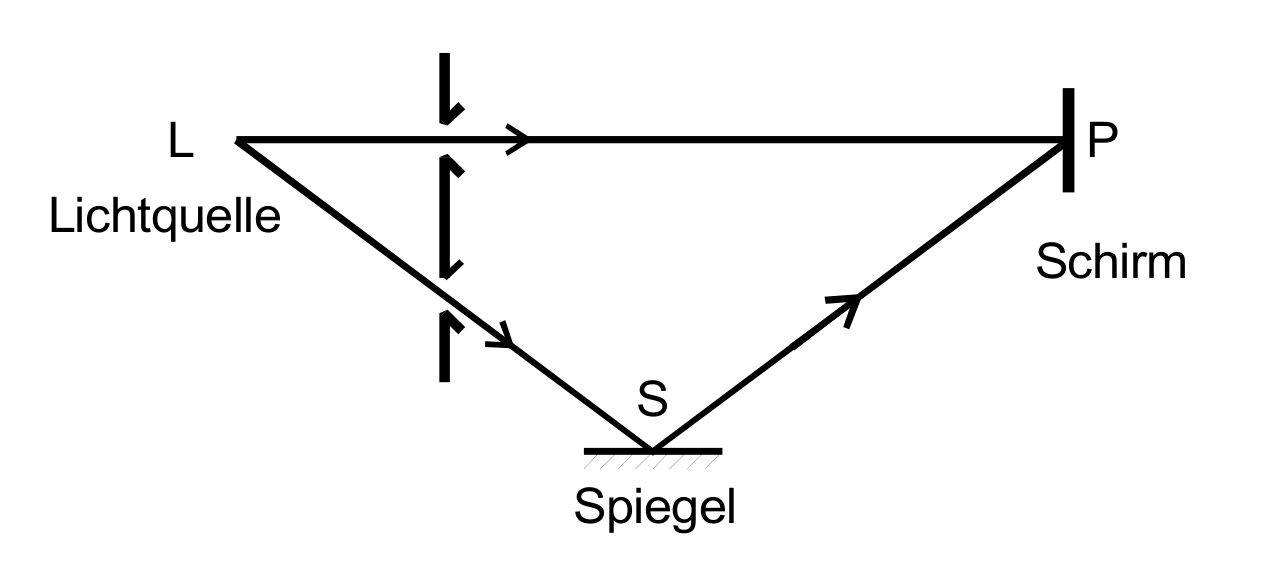
\includegraphics[width=8cm]{data/abb1.png}
    \caption{Interferenzerzeugung mit einer gewönlichen Lichtquelle \cite{sample}.}
    \label{fig:abb1}
\end{figure}
\FloatBarrier
Die beiden Strahlen werden dann in einem Punkt P zusammengeführt, wobei sie verschieden lange Wege zurück gelegt haben.
Dadurch besitzen sie eine Phasendifferenz, welche für die Interferenz sorgt.
Allerdings sind durch die Kohärenzlänge $l$ nicht immer Interferenzeffekte zu erkennen.
Der Emissionsvorgang dauert nur endlich lang, also besitzt die Welle auch nur eine endliche Länge.
Ist der Wegunterschied länger als die die Größe des Lichtzugs, dann kann keine Interferenz mehr entstehen, weil die Strahlen zu verschiedenen Zeiten eintreffen.
Die Kohärenzlänge $l$ ist genau die Länge bei der die Interferenz im Punkt P verschwindet.
Es gilt der Zusammenhang zwischen den maximal beobachteten Interferenzmaxima $N$ im Punkt P, der Wellenlänge $\lambda$ und der Kohärenzlänge $l$:
\begin{equation}
    l = N \lambda
\end{equation}

\subsection{Das Michelson-Interferometer}
\label{sec:theo2}

\begin{figure}
    \centering
    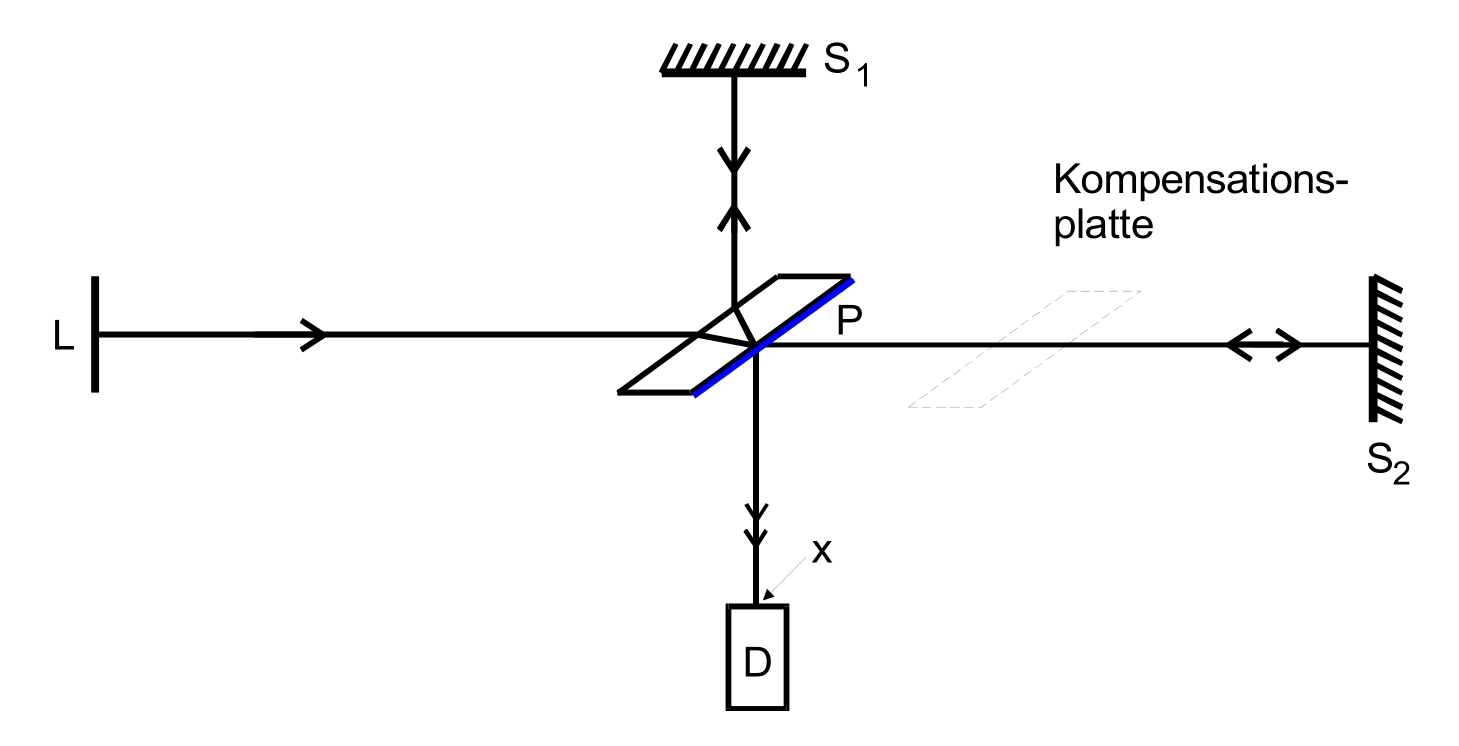
\includegraphics[width=8cm]{data/abb2.png}
    \caption{Michelson-Interferometer \cite{sample}.}
    \label{fig:abb2}
\end{figure}
\FloatBarrier
Es wird beim Michelson-Interferometer mittels eines semipermeablen Materials ein Lichtstrahl aufgespaltet, wie in Abbildung \ref{fig:abb1} zu sehen ist.
Ein Teil geht durch zum Spielgel $S_2$, der andere Teil wird zum Spiegel $S_1$ reflektiert.
Nach dem Reflektieren an beiden Spiegeln, treffen die Strahlen an der Platte P wieder zusammen und werden erneut geteilt.
Wichtig ist, dass beide Strahlen kohärnt sind.
Dafür werden die Abstände $\bar{S_1P} \text{ und } \bar{S_2P}$ fast gleich gewählt und in den Weg von $P$ zu $S_2$ wird eine Kompensationsplatte gestellt.
Diese gleicht die optische Weglänge der Strahlen aus, da der Strahl zu $S_1$ die Platte $P$ dreimal durchläuft, der Strahl zu $S_2$ allerdings nur einmal.
Wenn $\bar{S_1P} \text{ und } \bar{S_2P}$ gleichlang sind, dann ist an der Stelle $D$ ein Gangunterschied von $\frac{\lambda}{2}$, wodurch sich die Lichtstrahlen dann am Ort $D$ auslöschen.
Durch Verschiebung eines Spiegels um $\increment d$ ändert sich die Intensität des Interferenzmusters und man kann mit dem abgebildeten Aufbau die Wellenlänge $\lambda$ bestimmen mit
\begin{equation}
    \increment d = z \cdot \frac{\lambda}{2}
    \label{eqn:gl1}
\end{equation}
$z$ ist die Anzahl der beobachteten Interferenzmaxima. \\
Eine weitere Möglichkeit zur Erzeugung eines optischen Wegunterschiedes ist es,
einen der beiden Lichtstrahlen durch ein Medium der Länge b mit einem anderen Brechunsindex $n + \increment n$ laufen zu lassen, wie in Abbildung \ref{fig:abb3} zu sehen.
\begin{figure}
    \centering
    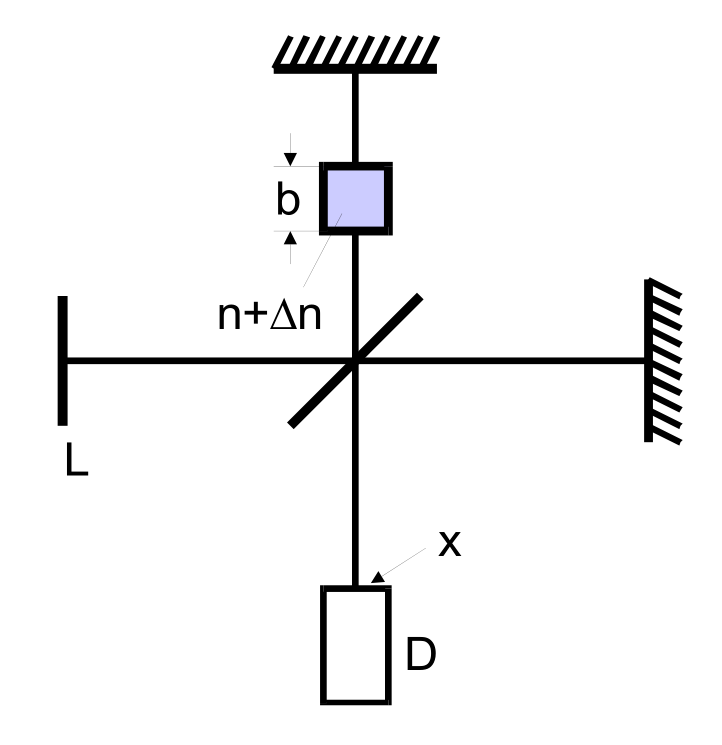
\includegraphics[width=5cm]{data/abb3.png}
    \caption{Aufbau zur Messung von Brechungsindexunterschieden \cite{sample}.}
    \label{fig:abb3}
\end{figure}
\FloatBarrier
Der Wegunterschied beträgt $\increment n b$.
Durch evakuieren oder erhöhen des Drucks $p$ in der Messzelle, lassen sich am Ort $D$ $z$ Interferenzen beobachten.
Es gilt die Formel:
\begin{equation}
    b \cdot \increment n = \frac{z \lambda}{2}
    \label{eqn:theo3}
\end{equation}
Es lässt sich zeigen, dass
\begin{equation}
    n = \sqrt{1+f(\lambda)N}
\end{equation}
gilt, wobei $N$ die Anazahl von Molekülen ist, die durch Lichtwellen der Wellenlänge zu Schwingungen angeregt werden.
Für Licht im sichtbaren Bereich lässt sich die Gleichung zu
\begin{equation}
    n = 1 + \frac{f}{2}N
\end{equation}
nähern.
Für die hier verwendeten Druckbereiche ist anzunehmen, dass sich die Gase wie ideale Gase verhalten.
Somit ist die Anzahl der Moleküle gegeben durch
\begin{equation}
    N(p,T) = \frac{p}{T} \frac{T_0}{p_0}N_L
\end{equation}
wobei $N_L$ die Loschmidtsche Zahl ist und $p_0$ und $T_0$ die Normalbedingungen sind.
Daraus ergibt sich für den Brechungsindexunterschied
\begin{equation}
    \increment n(p,p') = \frac{f}{2} N_L \frac{T_0}{p_0}\frac{1}{T}(p-p')
\end{equation}
Für den Brechungdindex unter Normalbedingungen gilt
\begin{equation}
    n(p_0,T_0) = 1 + \increment n(p,p') \frac{T}{T_0}\frac{p_0}{p-p'}
\end{equation}
$\increment n$ wird aus der umgestellten Gleichung \eqref{eqn:theo3} gewonnen, somit ergibt sich endgültig die Formel
\begin{equation}
    n(p_0,T_0) = 1 + \frac{z \lambda}{2b} \frac{T}{T_0} \frac{p_0}{p-p'}
    \label{eqn:gl2}
\end{equation}
